\section{Verdikonfigurasjons-analyse}
Verdikonfigurasjonsanalysen identifiserer sammensetningen av bedriftens aktiviteter og tilhørende verdi- og kostnadsdrivere \cite[s.~32]{FjeldstadogLunnan2018}. ROCKWOOL driver med industriell produksjon som er typisk for en verdikjede.

\begin{figure}[H]
\centering
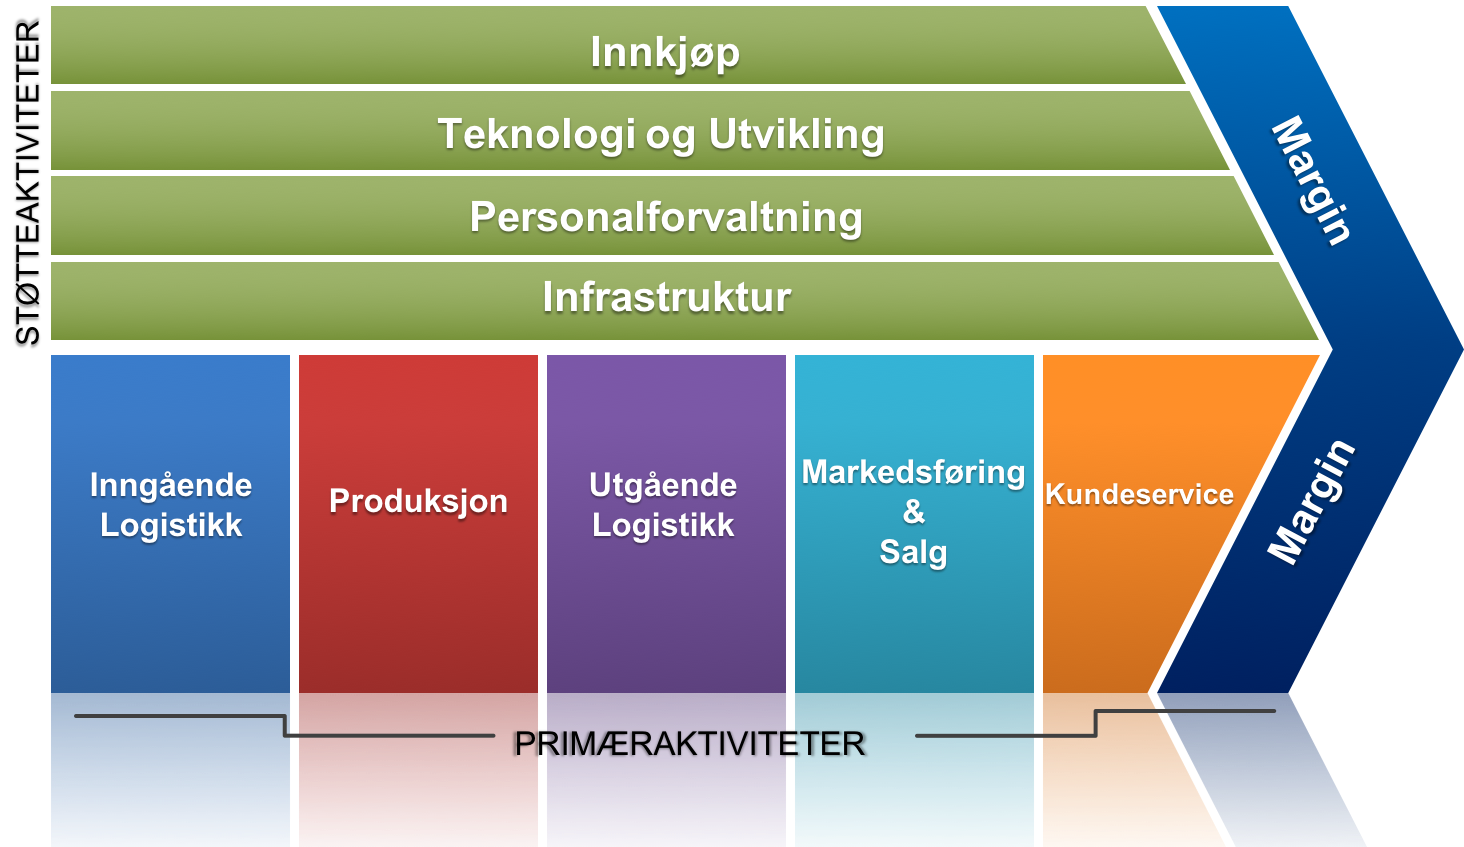
\includegraphics [scale=0.5]{bilder/verdikjede.png}
\caption{ROCKWOOL verdikjede}
\label{fig:verdikjede}
\end{figure}

\subsection{Primæraktiviteter}
Primæraktivitene er et sekvensielt sett av aktiviteter som direkte skaper verdi for kunden \cite[s.~132]{FjeldstadogLunnan2018}. 
 
\indent \newline
Som vist i figur \ref{fig:verdikjede} er den første aktiviteten inngående logistikk. Råvarer som vulkansk stein, koks og slagg (avfallsprodukter fra aluminiumsproduksjon) lagres, før det fraktes videre til produksjon. Her omformes innsatsfaktorene fra råvarer til steinull ved å bli utsatt for enormt høye temperaturer i en smelteovn. De ferdige produktene fraktes videre til lagring eller transporteres direkte til kunder avhengig av om det er produsert på bestilling. Markedsføring og salg fokuserer på byggevarekjeder og entreprenører. Det markedsføres derfor ikke direkte mot privatpersoner. Kundeservice består i hovedsak av teknisk service.

\indent \newline
ROCKWOOL har utfordringer med høye transportkostnader i forhold til andre konkurrenter grunnet hvor godt produktene lar seg komprimere. Produktene transporteres med lastebil ved fastprisavtale, og dårligere komprimering av produktene gir dermed lavere volum per transport. 

\subsection{Støtteaktiviteter}
Støtteaktivitetene skaper indirekte verdi for kunden gjennom sin effekt på primæraktivitetene \cite[s.~132]{FjeldstadogLunnan2018}. 

\subsubsection*{Innkjøp}
ROCKWOOL oppnår fordelaktige innkjøpsavtaler gjennom sin størrelse og store innkjøpskvantum, og blir videre forsterket gjennom sentral koordinering fra sitt konsern.

\subsubsection*{Teknologi og utvikling}
Både i AS ROCKWOOL og konsernet har de i mange år lagt mye ressurser i teknologiutvikling. De har tidligere utviklet sitt eget bindemiddel som gir energieffektiv og lydreduserende isolasjon, og dermed et konkurransedyktig produkt. I dag jobbes det med å forbedre komprimeringsegenskapene for å redusere kostnadene forbundet med transport.

\subsubsection*{Personalforvaltning}
De ansatte trives godt i jobben og føler tilhørighet til arbeidsoppgavene. Det er innarbeidet gode rutiner som sørger for at det er to personer med samme kompetanse til å utføre hver arbeidsoppgave. Dette sørger for en kontinuerlig flyt selv ved sykefravær og eventuelle oppsigelser.

\subsubsection*{Infrastruktur}
Vedlikehold og drift av produksjonen vurderes regelmessig etter KPIer (Key Performance Indicators). Dette er viktige nøkkeltall som ledelsen bruker for å evaluere måloppnåelse. Ledelsen har også tatt i bruk en Lean-metode som de kaller for Ropex. Metoden sørger for et kontinuerlig fokus på effektivitetsforbedringer.

\subsubsection*{Oppsummering}
ROCWOOL har i flere år jobbet med å effektivisere verdikjeden. Gjennom implementering av Ropex har bedriften tilegnet seg god kommunikasjon på tvers av avdelinger og kommandolinjer med fokus på å produsere mest mulig effektivt. På bakgrunn av dette, ser man lite rom for forbedring i verdikjeden. Det ligger imidlertid forbedringspotensial innenfor teknologiutvikling for å kunne forbedre kompaktheten til produktene og dermed øke volumet per transport.

\section{Verdikjedens drivere}
Verdikjedens drivere er strukturelle faktorer som påvirker verdiskapning for kunden og enhetskostnadene forbundet med å utføre aktivitetene \cite[s.~32]{FjeldstadogLunnan2018}. De viktigste driverne for ROCKWOOL er stordriftsfordeler og kapasitetsutnyttelse. Bedriften kan lagre produktene i opp til ett år før de må gjennom en ny kvalitetskontroll. Lang holdbarhet på produktene gir mulighet til å produsere i stor skala og dermed senke enhetskostnadene. Stordriftsfordelene forsterkes også av å være en del av ROCKWOOL-konsernet. Bedriften drar nytte av operasjonelle synergier gjennom gunstige prisavtaler hos leverandører ved å handle i stort kvantum.

\section{VRIO-analyse}
\begin{table}[ht]
\centering
\resizebox{\textwidth}{!}{%
\begin{tabular}{lccccc}
\hline
\rowcolor[HTML]{656565} 
{\color[HTML]{FFFFFF} \textbf{Ressurs}}                                                          & {\color[HTML]{FFFFFF} \textbf{Verdifull}} & {\color[HTML]{FFFFFF} \textbf{Sjelden}} & {\color[HTML]{FFFFFF} \textbf{Vanskelig å kopiere}} & {\color[HTML]{FFFFFF} \textbf{Effektivt organisert}} & {\color[HTML]{FFFFFF} \textbf{Avkastning}}     \\ \hline
\multicolumn{1}{|l|}{\cellcolor[HTML]{9B0000}{\color[HTML]{FFFFFF} \textbf{Finansiell kapital}}} & \multicolumn{1}{c|}{\cmark}                   & \multicolumn{1}{c|}{\xmark}                & \multicolumn{1}{c|}{\xmark}                            & \multicolumn{1}{c|}{\cmark}                              & \multicolumn{1}{c|}{\footnotesize Over gjennomsnittet}       \\ \hline
\multicolumn{1}{|l|}{\cellcolor[HTML]{9B0000}{\color[HTML]{FFFFFF} \textbf{Kompetanse}}}         & \multicolumn{1}{c|}{\cmark}                   & \multicolumn{1}{c|}{\cmark}                 & \multicolumn{1}{c|}{\cmark}                             & \multicolumn{1}{c|}{\cmark}                              & \multicolumn{1}{c|}{\footnotesize Over gjennomsnittet}       \\ \hline
\multicolumn{1}{|l|}{\cellcolor[HTML]{9B0000}{\color[HTML]{FFFFFF} \textbf{Teknologi}}}          & \multicolumn{1}{c|}{\cmark}                   & \multicolumn{1}{c|}{\xmark}                & \multicolumn{1}{c|}{\xmark}                            & \multicolumn{1}{c|}{\xmark}                             & \multicolumn{1}{c|}{\footnotesize Litt under gjennomsnittet} \\ \hline
\multicolumn{1}{|l|}{\cellcolor[HTML]{9B0000}{\color[HTML]{FFFFFF} \textbf{Produktegenskaper}}}  & \multicolumn{1}{c|}{\cmark}                   & \multicolumn{1}{c|}{\xmark}                & \multicolumn{1}{c|}{\cmark}                             & \multicolumn{1}{c|}{\cmark}                              & \multicolumn{1}{c|}{\footnotesize Over gjennomsnittet}       \\ \hline
\end{tabular}%
}
\caption{Ressursanalyse}
\label{ressursanalyse}
\end{table}

\subsection{Finansiell kapital}
ROCKWOOL har hatt en lønnsom drift i flere år og hadde i 2017 et årsresultat på 64 millioner kroner og en egenkapital på 382 millioner kroner \cite{ProffRegnskap}. I tillegg drar de nytte av finansielle synergier ved å være en del av et konsern. De står dermed godt rustet for potensielle investeringer i tiden fremover.

\subsection{Kompetanse}
Kompetansen anses som meget god. Turnover-raten er på bare 2\% og mange av de ansatte har en fartstid på 15-35 år i bedriften. For å fortsette kompetanseutviklingen blant de ansatte har de innarbeidet interne opplærings- og utdanningssystemer. Bedriften bør imidlertid være oppmerksom på at kompetanse kan forsvinne i årene som kommer på grunn av en relativt høy gjennomsnittsalder.

\subsection{Teknologi}
Det investeres mye ressurser i teknologi, både i ROCKWOOL og konsernet. Utvikling av egne smelteovner har tidligere gitt konkurransefortrinn i markedet, men med dagens smelteteknologi henger de etter de største konkurrentene med tanke på å produsere miljøvennlig. Å redusere CO2-utslipp i forbindelse med produksjonsprosessen anses som kritisk for å kunne være konkurransedyktige i fremtiden.

\subsection{Produktegenskaper}
Steinull innehar flere egenskaper og bruksområder enn de fleste andre isolasjonsproduktene i markedet. Produktet isolerer, er vannavstøtende, har lyddempende egenskaper og er en god kilde til brannsikring. Det er kun ROCKWOOL og Paroc som scorer høyt på alle disse produktattributtene, mens andre aktører kun leverer på to av punktene.

\subsection{Oppsummering}
Analysen viser at ROCKWOOL har konkurransefortrinn i produktegenskapene. Dette anses som langvarig da egenskapene kommer naturlig fra råvaren i kombinasjon med et egetutviklet bindemiddel. Det vil også være kostbart for andre aktører å bytte til steinullproduksjon i form av store investeringer og mangel på erfaring. Fremover vil det være viktig å utvikle og investere i ny miljøvennlig smelteteknologi som jeg anser som en av bedriftens største utfordringer i dag.